\section{Convolutional Neural Networks}
\label{sec:cnn}
A Convolutional Neural Network (CNN) is a particular type of Artificial Neural Network (ANN). Similarly to an ANN, it receives an input and returns an output, through a series of hidden layers. Furthermore, it learns its parameters by minimising an error function, usually by performing backpropagation. 

As opposed to an ANN, where each input is typically fully connected with neurons of the next layer, a CNN instead has sparse connectivity. Each neuron in the hidden layer is connected only to a local part of the input and output. In a high-dimensional scenario full connectivity would yield an extremely large number of parameters, leading to overfitting.

Often, CNNs make the assumption that the inputs are images, constraining the architecture of the layers in 3 dimensions: \textit{width}, \textit{height}, \textit{depth}. An illustration of the structure is given below:

\begin{figure}[htbp]
	\centering
	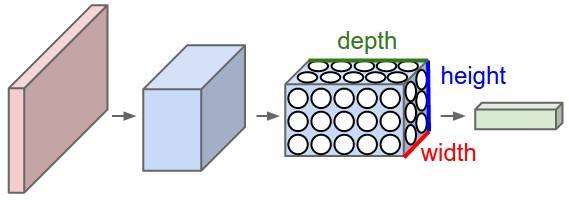
\includegraphics[scale=0.5]{cnn.png}
	\caption{The architecture of a CNN, where each layer is organised in three dimensions. Notice that each layer transforms a 3D input to a 3D output. Graphic sourced from \cite{CS231n}.}
	\label{CNN}
\end{figure}
\vspace{0.3cm}
A CNN is represented as a list of layers, where each layer transforms an input volume to an output volume through a differentiable function. There are distinct type of layers and activation functions; a typical structure could contain:
\begin{itemize}
	\item \textbf{Input} - a representation of the input image, for example a [128x128x3] volume for an image of width 128, height 128 and 3 channels for the colors RGB. 
	\item \textbf{Convolution} - an operation convolving a set of weights with the input volume; this is done by performing dot products between local regions and the weights. As a result we obtain another volume, for example of size [128x128x12]. The depth parameter is analogous to the number of hidden layers in ANN, and it controls the number of neurons in the convolution layer that connect the same local region of the input volume. 
	\item \textbf{ReLU} - a function that performs elementwise activation of the component of the volume, specifically $\max(0, x)$. Notice that in this stage the dimension of the volume is unchanged. 
	\item \textbf{Max Pooling} - a layer that reduces the dimension of the image (width and height), by selecting the maximum entry of a given region. This effectively downsamples the volume in the spatial dimensions.
	\item \textbf{Fully connected} - a layer in which each neuron is connected to all neurons of the previous layer as in an ANN, without weight-sharing or sparsity.
\end{itemize}

In this way, a CNN converts the original input image to the final category score, layer by layer. In the same way as an ANN, the parameters of the network can be trained with gradient descent.

Building an efficient CNN involves choosing the configuration of layers. Firstly, the \textit{depth} of convolution layers must be chosen; controlling the number of neurons that connect to the same region of the input volume. 
Secondly, we need to fix the \textit{receptive field}, which is the size of the local region of the input that we will convolve. Thirdly, we have to specify the \textit{stride} with which the receptive field will look at the input image; the bigger the stride, the smaller the output volume. Finally,  it is sometimes necessary to pad the input volume with zeros along the borders; so we also need to specify this parameter, called \textit{padding} that allow us to control the spatial size of the output volume. 

